\begin{figure}[!hp]
  \begin{center}
      \begin{tikzpicture}
        \begin{axis}[
            hide axis,
            %colorbar,
             scale only axis,
             height=0.26\rasterimagewidth,,
             width=\rasterimagewidth,
             %colorbar horizontal,
             point meta min=2.38,
             point meta max=4.21,
             colorbar style={
               title=Concentration [\%w],
               width=7.4cm,
               height=0.3cm,
               xtick={2.38, 3, 3.5, 4,4.21, 4.5, 5, 5.5, 6},
               at={(0.5\rasterimagewidth,0.4cm)},
               anchor=north
            }
          ]
          \addplot [] coordinates {(0,0)};
          \node (myfirstpic) at (0,0) {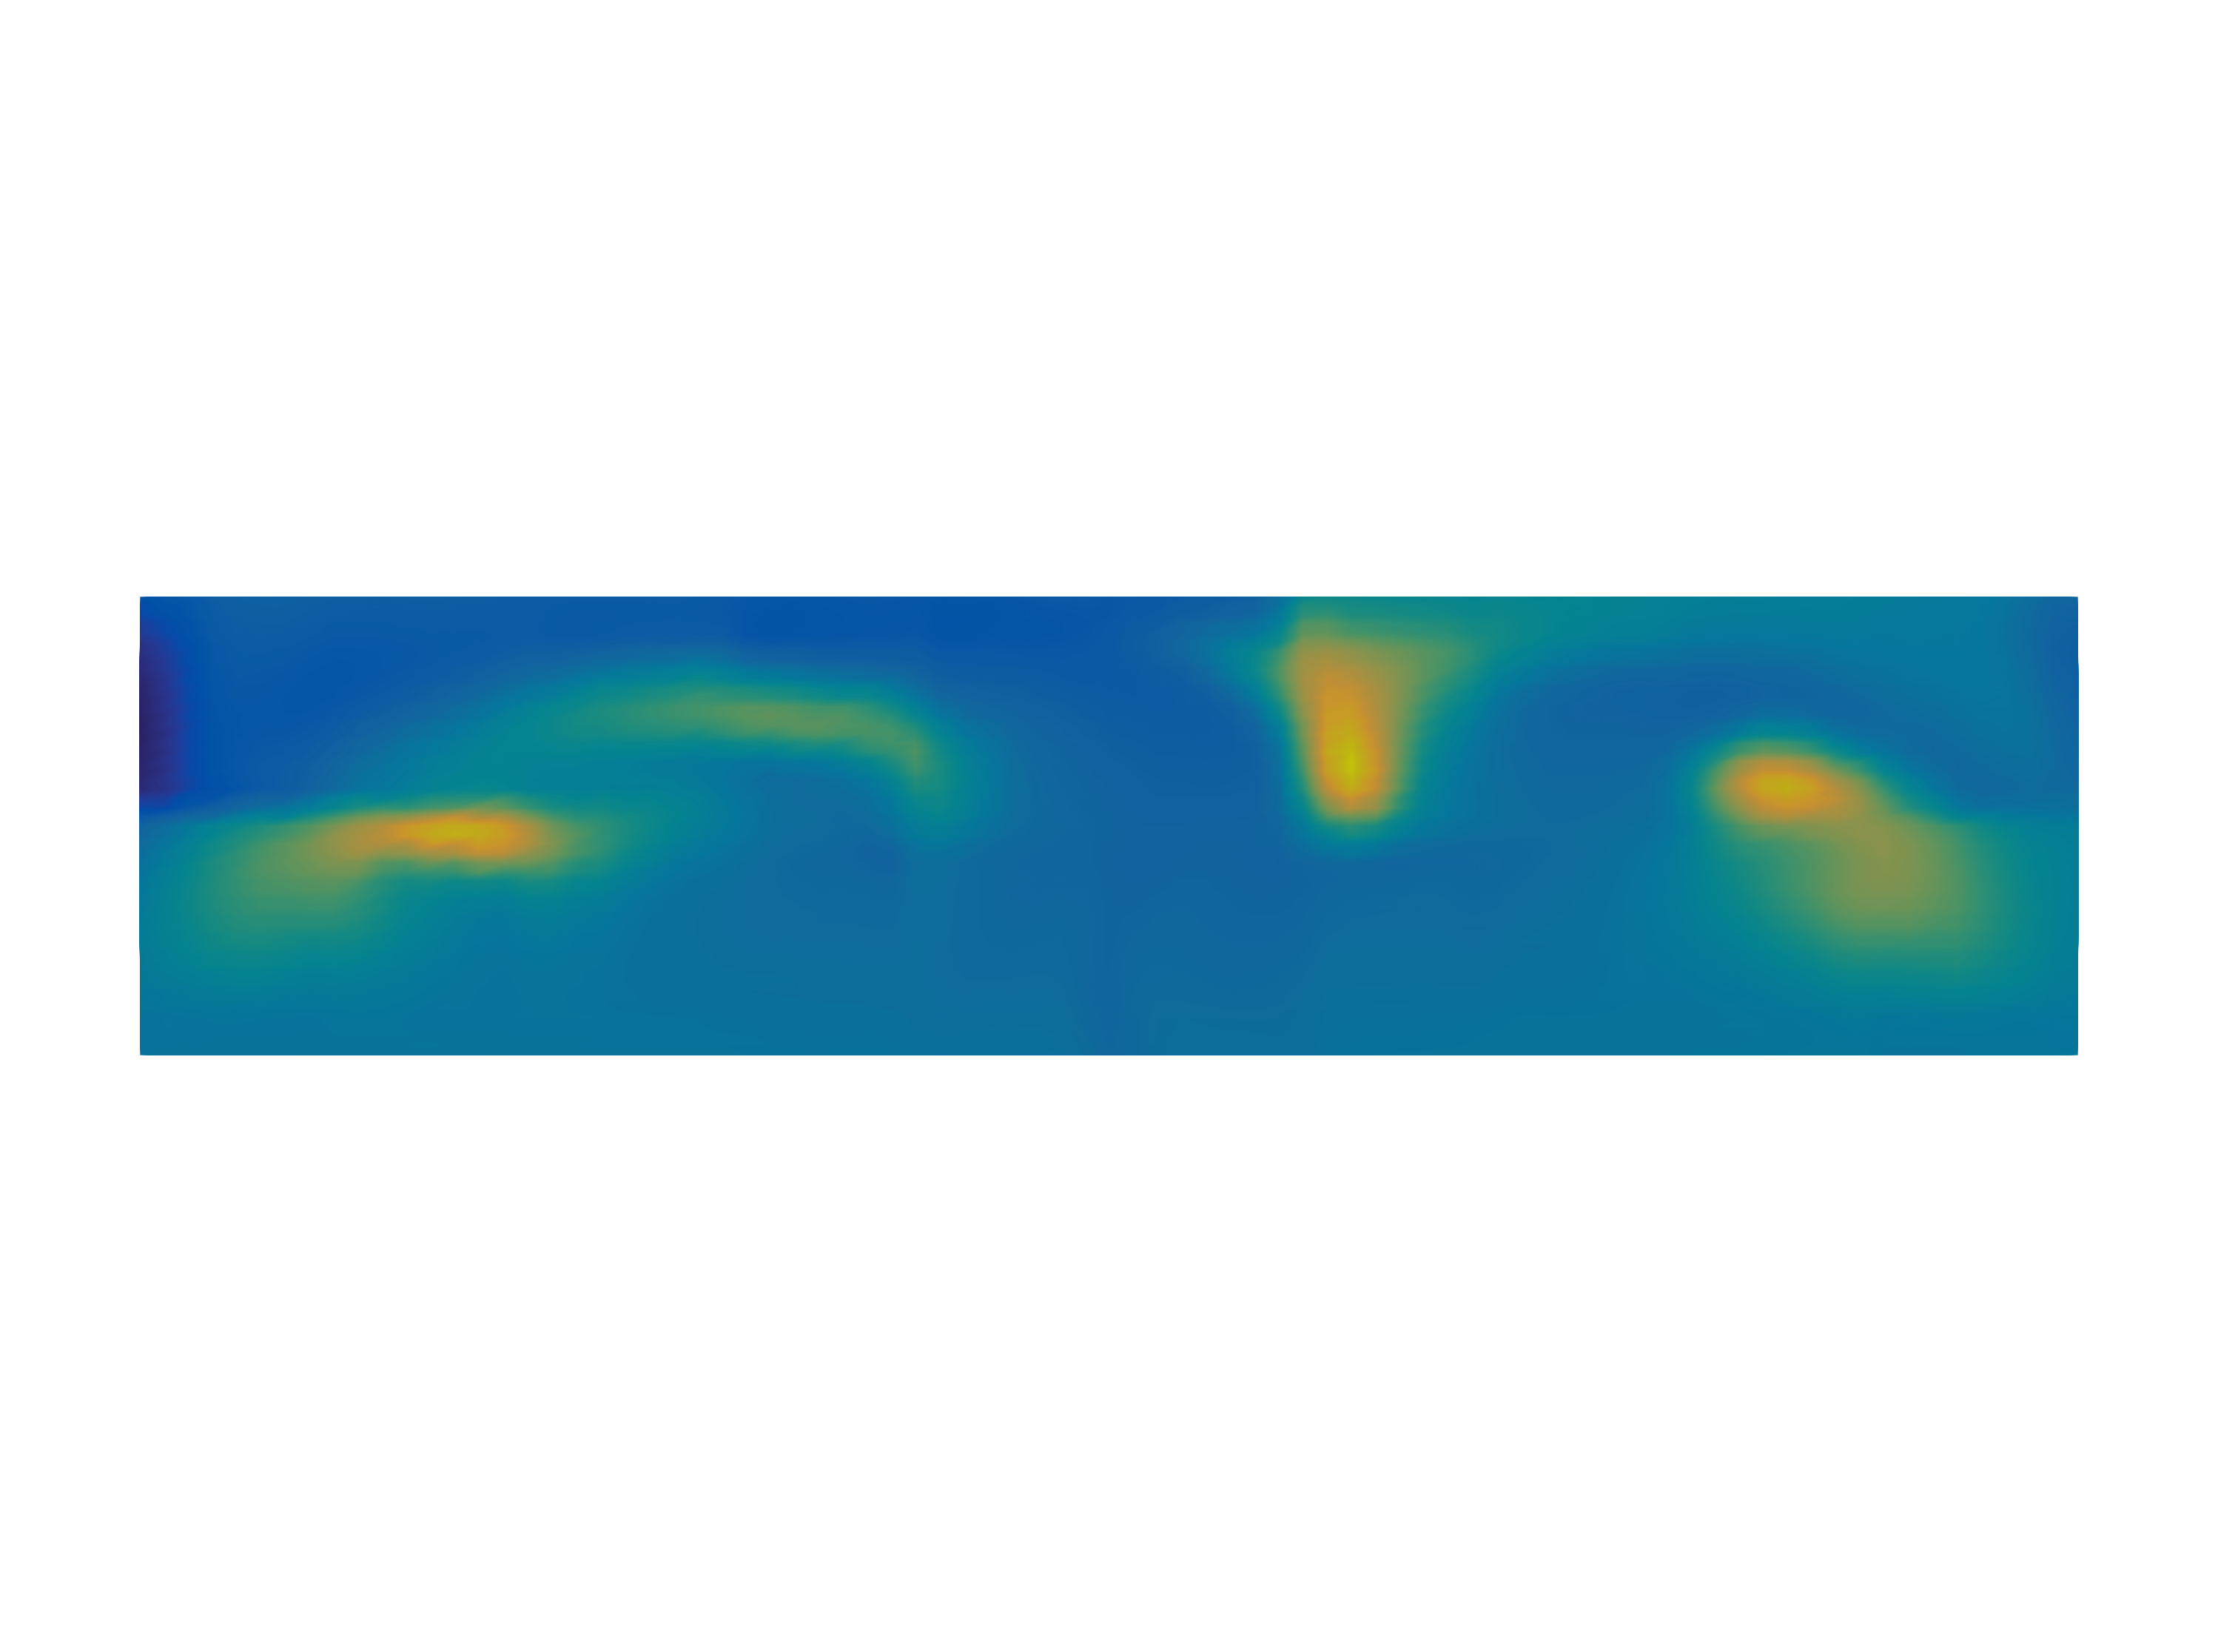
\includegraphics[width=\rasterimagewidth]{{../media/populations/application/print/alumina-control-2.38-4.21}.png}};
        \end{axis}
      \end{tikzpicture}
      \begin{tikzpicture}
        \begin{axis}[
            colorbar,
            hide axis,
            scale only axis,
            height=0.52\rasterimagewidth,
            width=\rasterimagewidth,
            colorbar horizontal,
            point meta min=2.38,
            point meta max=4.21,
            colorbar style={
              title=Concentration [\%w],
              width=7.4cm,
              height=0.3cm,
              xtick={2.38, 3, 3.5, 4,4.21, 4.5, 5, 5.5, 6},
              at={(0.5\rasterimagewidth,3.0cm)},
              anchor=north
            }
          ]
          \addplot [] coordinates {(0,0)};
          \node (myfirstpic) at (0,50) {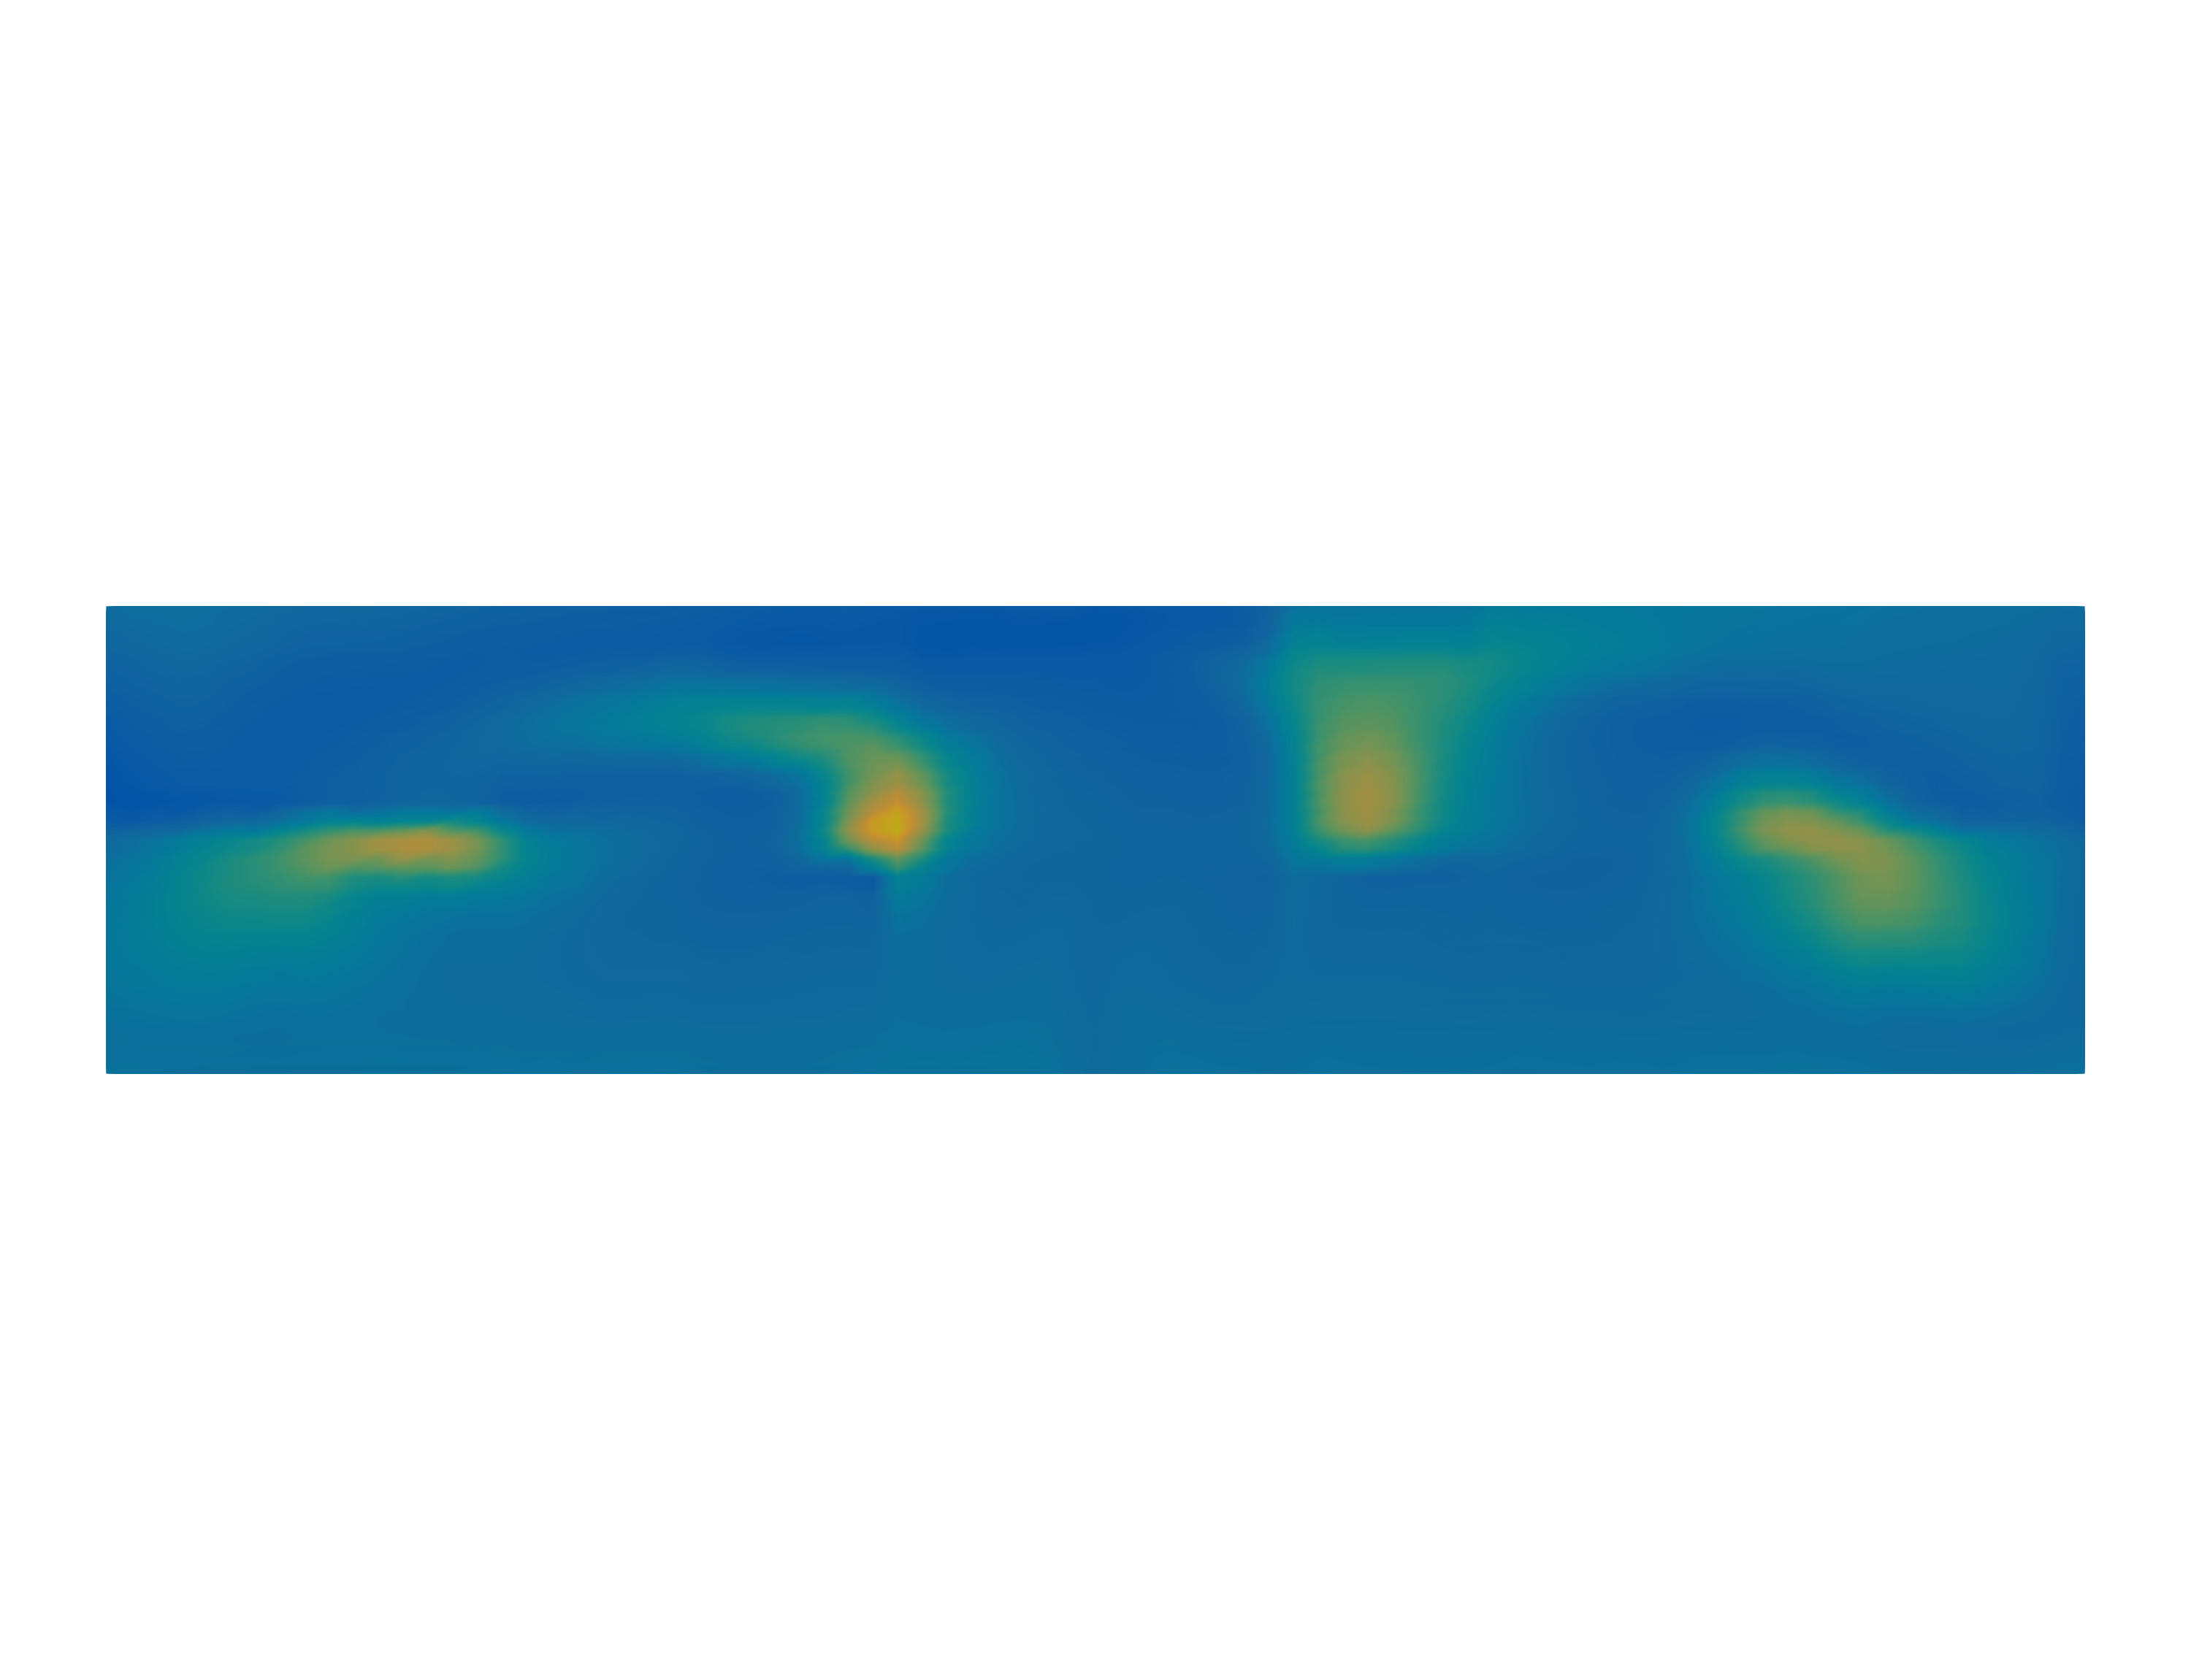
\includegraphics[width=\rasterimagewidth]{{../media/populations/application/print/dummy-tmp-result-c-2.38-4.21}.png}};
        \end{axis}
      \end{tikzpicture}
      \caption{Champ de concentration d'alumine dissoute dans l'ACD de
        la cuve AP32 à $t = \num{10000}\si\second$. En haut,
        dissolution des particules sans chute gravitationnelle dans le
        bain. En bas, dissolution des particules avec chute
        gravitationnelle dans le bain.}
      \label{fig:sedimentation-comparaison}
  \end{center}
\end{figure}
